%XeLaTeX+makeIndex+BibTeX

\documentclass[a4paper,12pt]{article} %14pt - extarticle
\usepackage[utf8]{inputenc} %русский язык, не менять
\usepackage[T2A, T1]{fontenc} %русский язык, не менять
\usepackage[english, russian]{babel} %русский язык, не менять
\usepackage{hyperref} %гиперссылки
\hypersetup{pdfstartview=FitH,  linkcolor=black, urlcolor=black, colorlinks=false} %гиперссылки
\usepackage{graphicx} %изображения
\usepackage{float}%картинки где угодно
\usepackage{textcomp}
\usepackage{fancyvrb} %fancy verbatim for \VerbatimInput
\usepackage{dsfont}%мат. символы
\usepackage{amsmath, mathtools} %common math symbols
\newcommand{\norm}[1]{\left\lVert#1\right\rVert}
\usepackage{listings} %code formatting
\usepackage[linesnumbered, ruled]{algorithm2e}%pseudocode 
\SetKwRepeat{Do}{do}{while}
\lstset{language=python,
	%keywordstyle=\color{black},
	%commentstyle=\color{},
	%stringstyle=\color{red},
	tabsize=1,
	breaklines=true,
	columns=fullflexible,
	%numbers=left,
	escapechar=@,
	morekeywords={numpy, np}
}

\textwidth=16cm
\oddsidemargin=0cm %поля (отступ слева)
\topmargin=-1cm %поля (отступ сверху)
\textheight=23cm

\begin{document}
	\begin{titlepage}
		\begin{center}
			\begin{large}
				Санкт-Петербургский политехнический университет Петра Великого\\
				Институт прикладной математики и механики\\
				\textbf{Кафедра <<Прикладная математика>>}\\
			\end{large}
			\vfill
			\Large{\textbf{КУРСОВАЯ РАБОТА\\
					ПО ДИСЦИПЛИНЕ <<МАТЕМАТИЧЕСКАЯ СТАТИСТИКА>>}}
		\end{center}
		\vfill
		\flushleft
		Выполнил\\
		студент группы $3630102/70301$
		\flushright
		Камянский Д.В.\\
		\flushleft
		Проверил\\
		к. ф.-м. н., доцент\\
		\flushright
		Баженов А.Н.
		\vfill
		\centering{Санкт-Петербург \\ 2020}
	\end{titlepage}

	\section{Постановка задачи}

	\subsection{Подготовка данных}
	\begin{itemize}
		\item Cчитать данные светимости;
		\item Выделить временные интервалы с различным типом циклического движения;
		\item Разделить матрицы состояния плазы по соответсвующим временым интервалам.
	\end{itemize}
	
	\subsection{Расчеты}
	\begin{itemize}
		\item Расчитать положение центра масс системы для каждого момента времени;
		\item Рассчитать периоды прохождения центром масс циклической траектории и соответсвующую частоту движения;
		\item Расчитать значения характерезующие частоту движения центра масс.
	\end{itemize}
	
	\subsection{Анализ}
	Рассмотреть характер вращения системы и зависимость частоты вращения от времени.
	
	
	\section{Теория}
	\subsection{Центр масс}
	Центр масс - геометрическая точка, характеризующая движение тела или системы частиц как целого. 
	Положение центра масс системы определяется следующим образом:
	\begin{equation}
	r_{c}= \frac{\sum m_{i}r_{i}}{\sum m_{i}}
	\end{equation}
	где $r_{c}$ - радиус-вектор центра масс, $r_{i}$ -  радиус-вектор $i$-й точки системы, $m_{i}$ - значение светимости в $i$-й точке.
	
	\subsection{Выборочная медиана и выборочное среднее}
	Выборочная медиана - это значение, которое разбивает выборку на две равные части. Половина наблюдений лежит ниже медианы, и половина наблюдений лежит выше медианы.
	Медиана вычисляется следующим образом. Изучаемая выборка упорядочивается в порядке возрастания (N - объем выборки). Получаемая последовательность $a_{k}$, где $k=1,...,N$ называется вариационным рядом или порядковыми статистиками. Если число наблюдений $N$ нечетно, то медиана оценивается как $m=a_{\frac{N+1}{2}}$.
	Если число наблюдений N четно, то медиана оценивается как $m=(a_{\frac{N}{2}} + a_{\frac{N}{2} + 1})$
	\newline Пусть $X_{1}, ..., X_{n}$ - выборка. Среднее значение выборки оценивается по формуле: $\overline{X}= \frac{\sum_{i=1}^{n}X_{i}}{n}$.
	
	\subsection{Выборочный коэффициент корреляции Пирсона}
	Пусть по выборке значений $\{x_{i},y_{i}\}^{n}_{1}$ двумерной с.в. (X,Y ) требуется оценить коэффициент корреляции $\rho = \frac{cov(X,Y)}{\sqrt{DXDY}}$ . Естественной оценкой для $\rho$ служит его статистический аналог в виде выборочного коэффициента корреляции, предложенного К.Пирсоном, —
	\begin{equation}
	r = \frac{
		\frac{1}{n}\sum{(x_{i} - \bar{x})(y_{i}-\bar{y})}
	}{
		\sqrt{\frac{1}{n}\sum{(x_{i} - \bar{x})^{2}}\frac{1}{n}\sum{(y_{i} - \bar{y})^{2}}}
	}=\frac{K}{s_{X}s_{Y}},
	\label{r}
	\end{equation}
	где $K,s^{2}_{X},s^{2}_{Y}$ — выборочные ковариация и дисперсии с.в. X и Y [1, c. 535].
	\section{Реализация}
	Лабораторная работа выполнена с помощью встроенных средств языка программирования Python в среде разработки JupyterLab. Использованы библиотеки scipy для загрузки данных из файла, numpy для простоты использования различных статистических функций,matplotlib и seaborn для визуализации результатов.
	Исходный код лабораторной работы приведён в приложении в виде ссылки на репозиторий GitHub.
	\section{Результаты и Анализ полученных данных}
	На видео движения светимости плазмы можно выделить 2 интервала: интервал вращения ([157.0, 167.0]), где чётко разлечимо вращение ядра (область с самыми высокими значениями светимости):
	\begin{figure}[H]
		\centering
		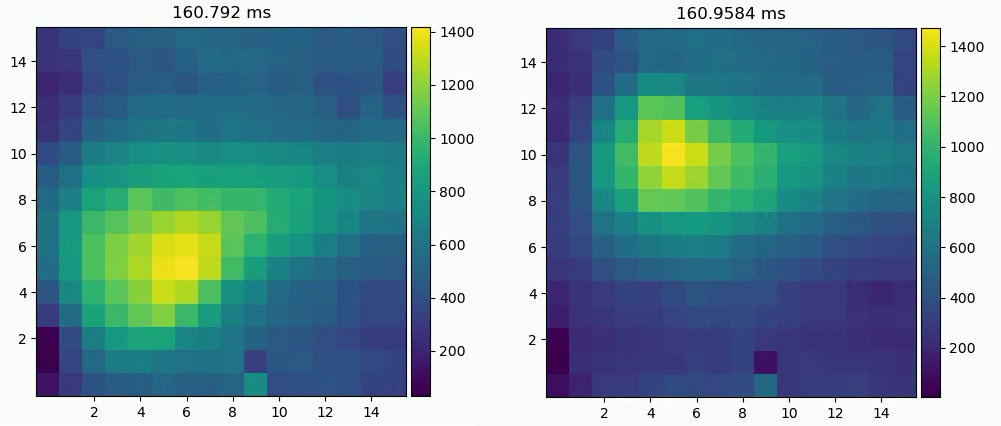
\includegraphics[width = 18cm, height = 12cm]{Rot_prj.png}
		\caption{Интервал вращения [157.0, 167.0]}
		\label{fig:rot_prj}
	\end{figure}
	и интервал колебания ([167.0, 175.0]), где ядро либо остаётся на месте, либо отклоняется очень незначительно от изначального положения и быстро к нему возвращается:
	\begin{figure}[H]
		\centering
		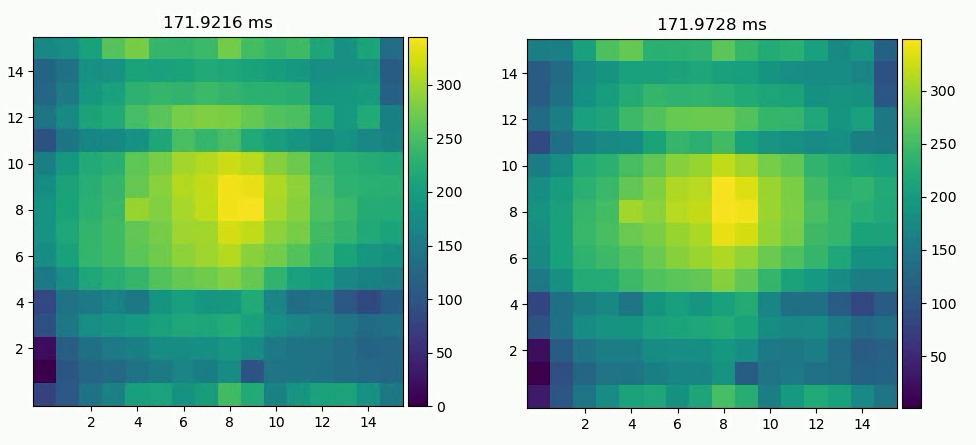
\includegraphics[width = 18cm, height = 12cm]{Fluct_prj.png}
		\caption{Интервал колебания [167.0, 175.0]}
		\label{fig:fluct_prj}
	\end{figure}
	Для исследования движения (в частности вращения) системы используется исследование движения центра масс. Частота расчитывается по формуле $\nu = \frac{1}{T}$, где $T$ - период обращения центра масс (время, за которое точка центра масс возвращается в стартовое положение начала периода).
	\subsection{Частота вращения системы по исходным данным}
	\begin{figure}[H]
		\centering
		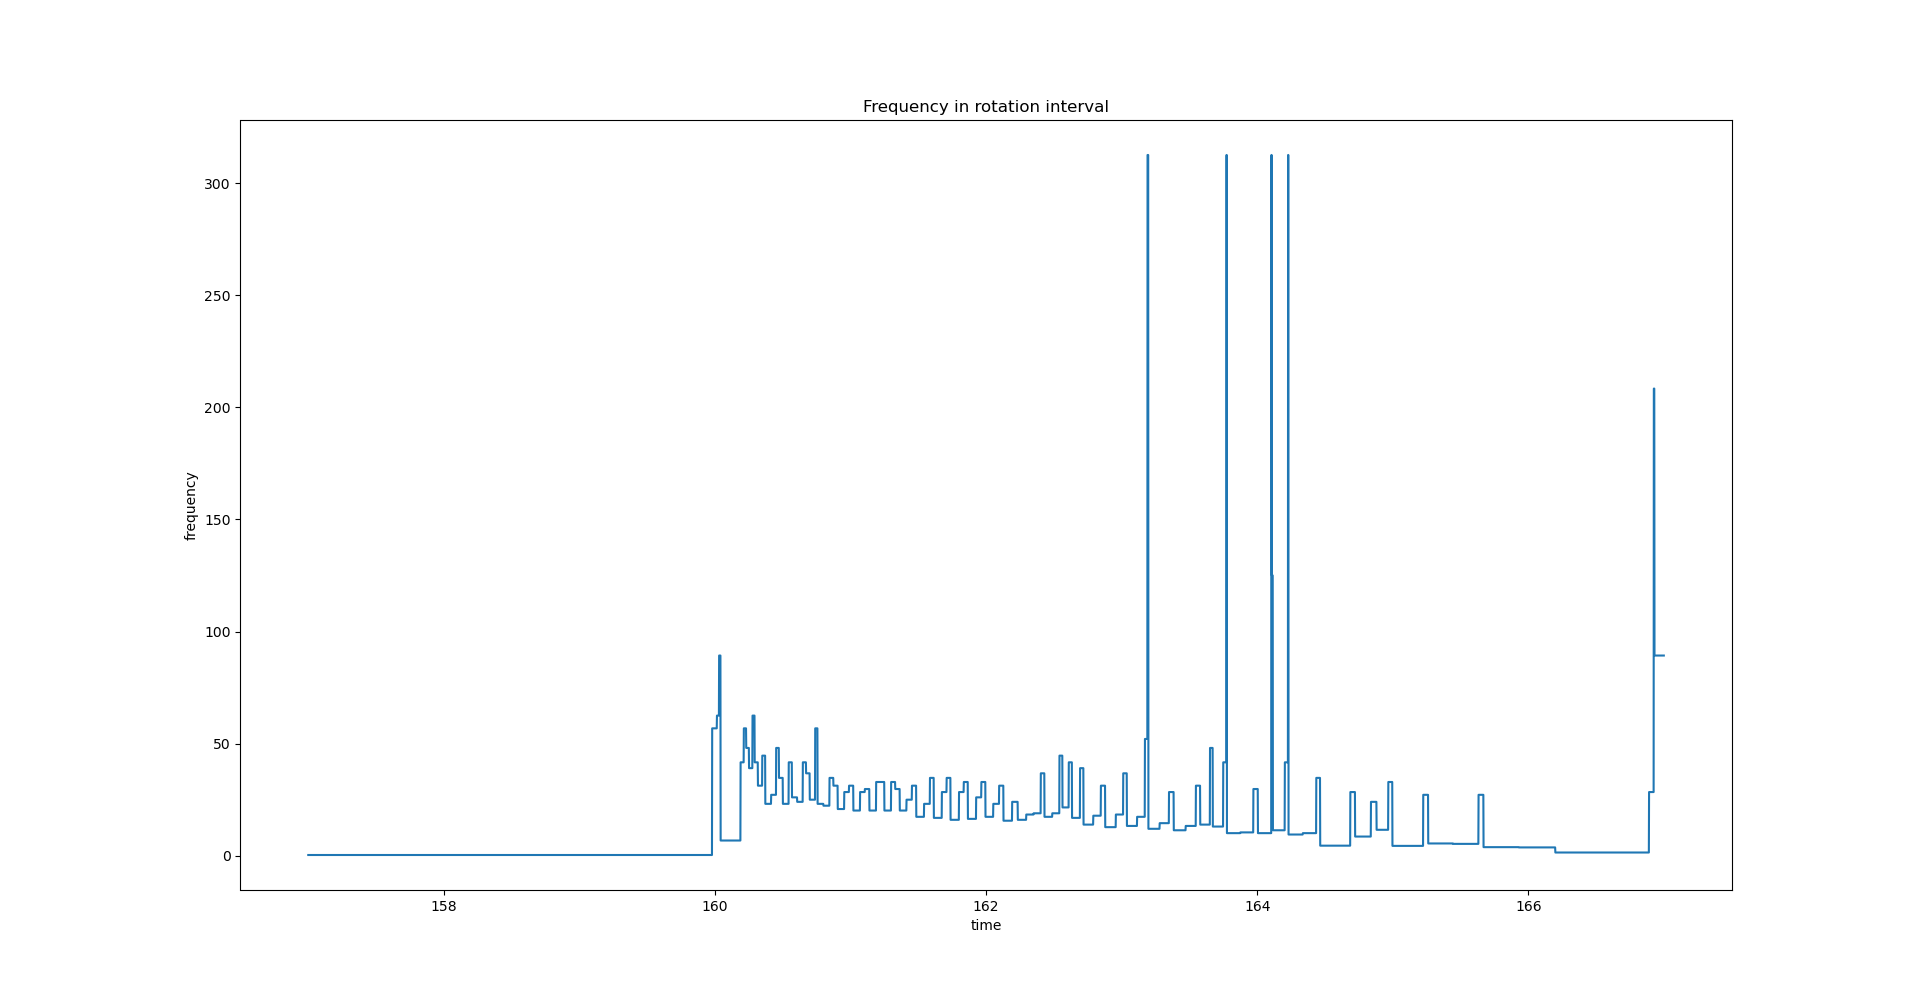
\includegraphics[width = 18cm, height = 12cm]{Rot_origin.png}
		\caption{Частота вращения системы на интервале вращения [157.0, 167.0]}
		\label{fig:rot_origin}
	\end{figure}
	\begin{figure}[H]
		
		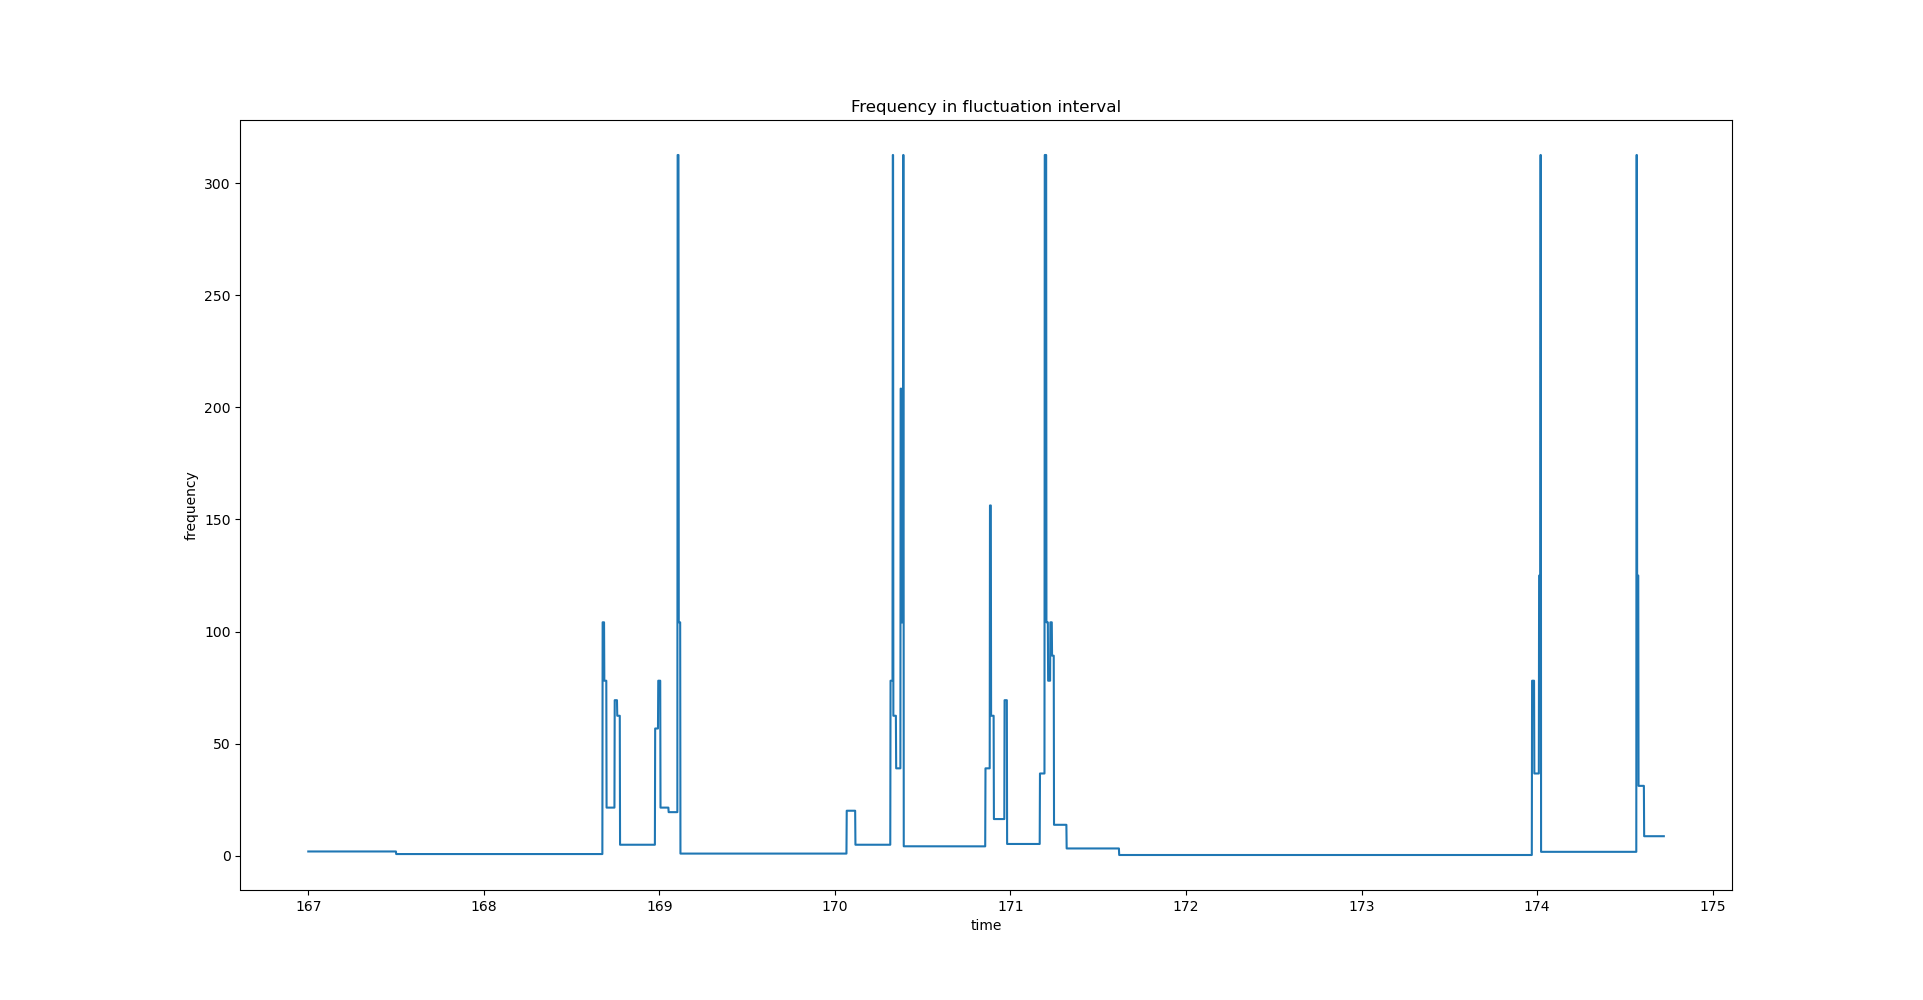
\includegraphics[width = 18cm, height = 12cm]{Fluct_origin.png}
		\caption{Частота вращения системы на интервале колебаний [167.0, 175.0]}
		\label{fig:fluct_origin}
	\end{figure}

	\begin{table}[H]
		\caption{Соотношение кол-ва вариаций позиции центра масс с кол-ом временных промежутков}
		\label{tab:my_label1}
		\begin{center}
			\vspace{5mm}
			\begin{tabular}{|c|c|c|}
				\hline
				 & Вращение & Колебания\\
				\hline
				Кол-во различных позиций ц.м. & $ 248 $ & $ 106 $\\
				\hline
				Кол-во временных промежутков & $ 6250 $ & $ 5000 $\\
				\hline
			\end{tabular}
		\end{center}
	\end{table}
	
	\begin{table}[H]
		\caption{Выборочные характеристики частоты вращения}
		\label{tab:my_label2}
		\begin{center}
			\vspace{5mm}
			\begin{tabular}{|c|c|c|}
				\hline
				& Среднее & Медиана\\
				\hline
				Вращение & $ 12.93 $ & $ 5.48 $\\
				\hline
				Колебания & $ 6.86 $ & $ 1.06 $\\
				\hline
			\end{tabular}
		\end{center}
	\end{table}

	Коэффициент корреляции Пирсона между частотой вращения и временем на интервале вращения $r = 0.1461$.
	\newline Продолжительные пологие участки графиков - это временные промежутки на которых центр масс длительное время не меняет положения внутри цикла вращения (колебания), что приводит к сильному увеличению периода оборота. Данная проблема хорошо прослеживается при соотношении кол-ва различных позиций центра масс и количества рассматриваемых временных промежутков. Видно что большей части времени центр масс не меняет своей позиции.
	\newline Чтобы преодолеть проблему низкой изменчивости позиции центра масс, были рассмотрены два подхода: слабая фильтрация с последующим ослаблением ядра и сильная фильтрация.
	
	\subsection{Частота вращения системы после слабой фильтрации и ослабления ядра}
	Данный подход опирается на предположение, что причиной малой изменчивости позиции центра масс (далее ц.м.) является малая подвижность ядра системы и чтобы увеличить вес хвостовой части вращения требуется ослабить центральную ядерную часть. Чтобы при подобном ослаблении не увеличивать весовую роль шумовых значений, предварительно отфильтруем систему на значения меньшие или равные 25-му перцентилю.
	\begin{figure}[H]
		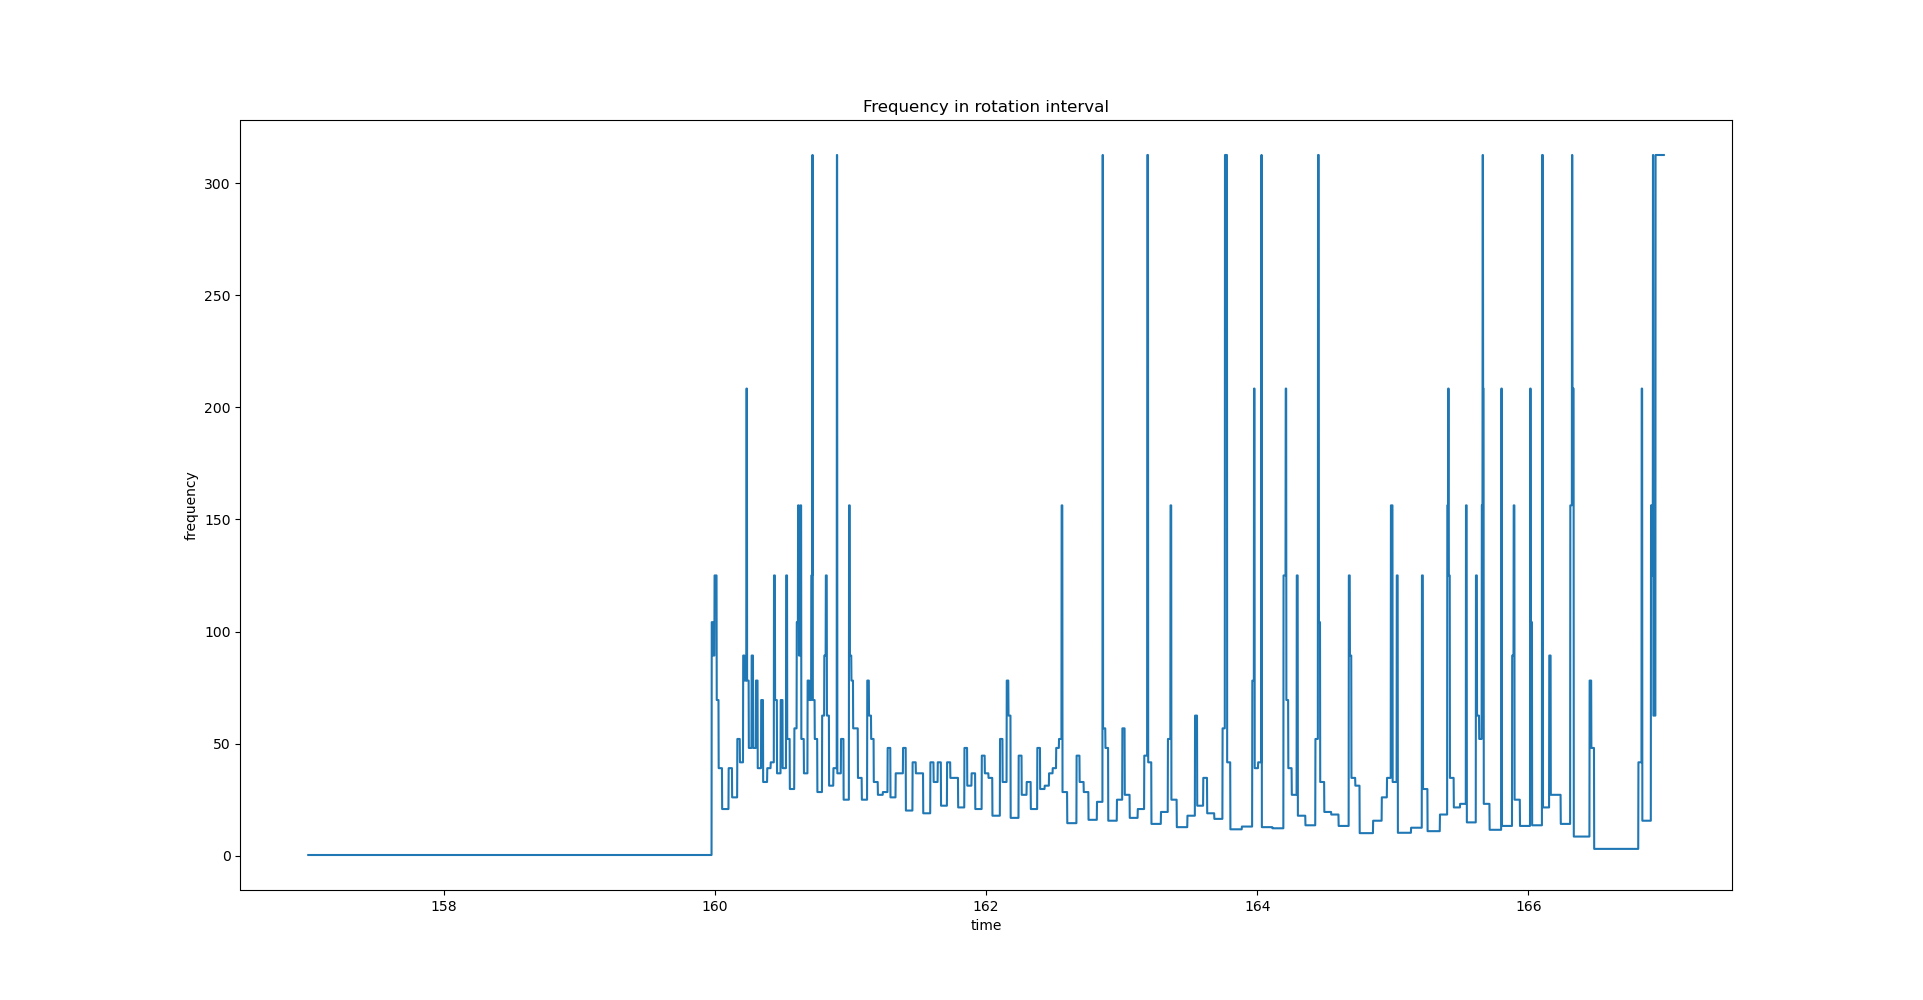
\includegraphics[width = 18cm, height = 12cm]{Rot_dropped.png}
		\caption{Частота вращения системы на интервале вращения [157.0, 167.0]}
		\label{fig:rot_dropped}
	\end{figure}
	\begin{figure}[H]
		
		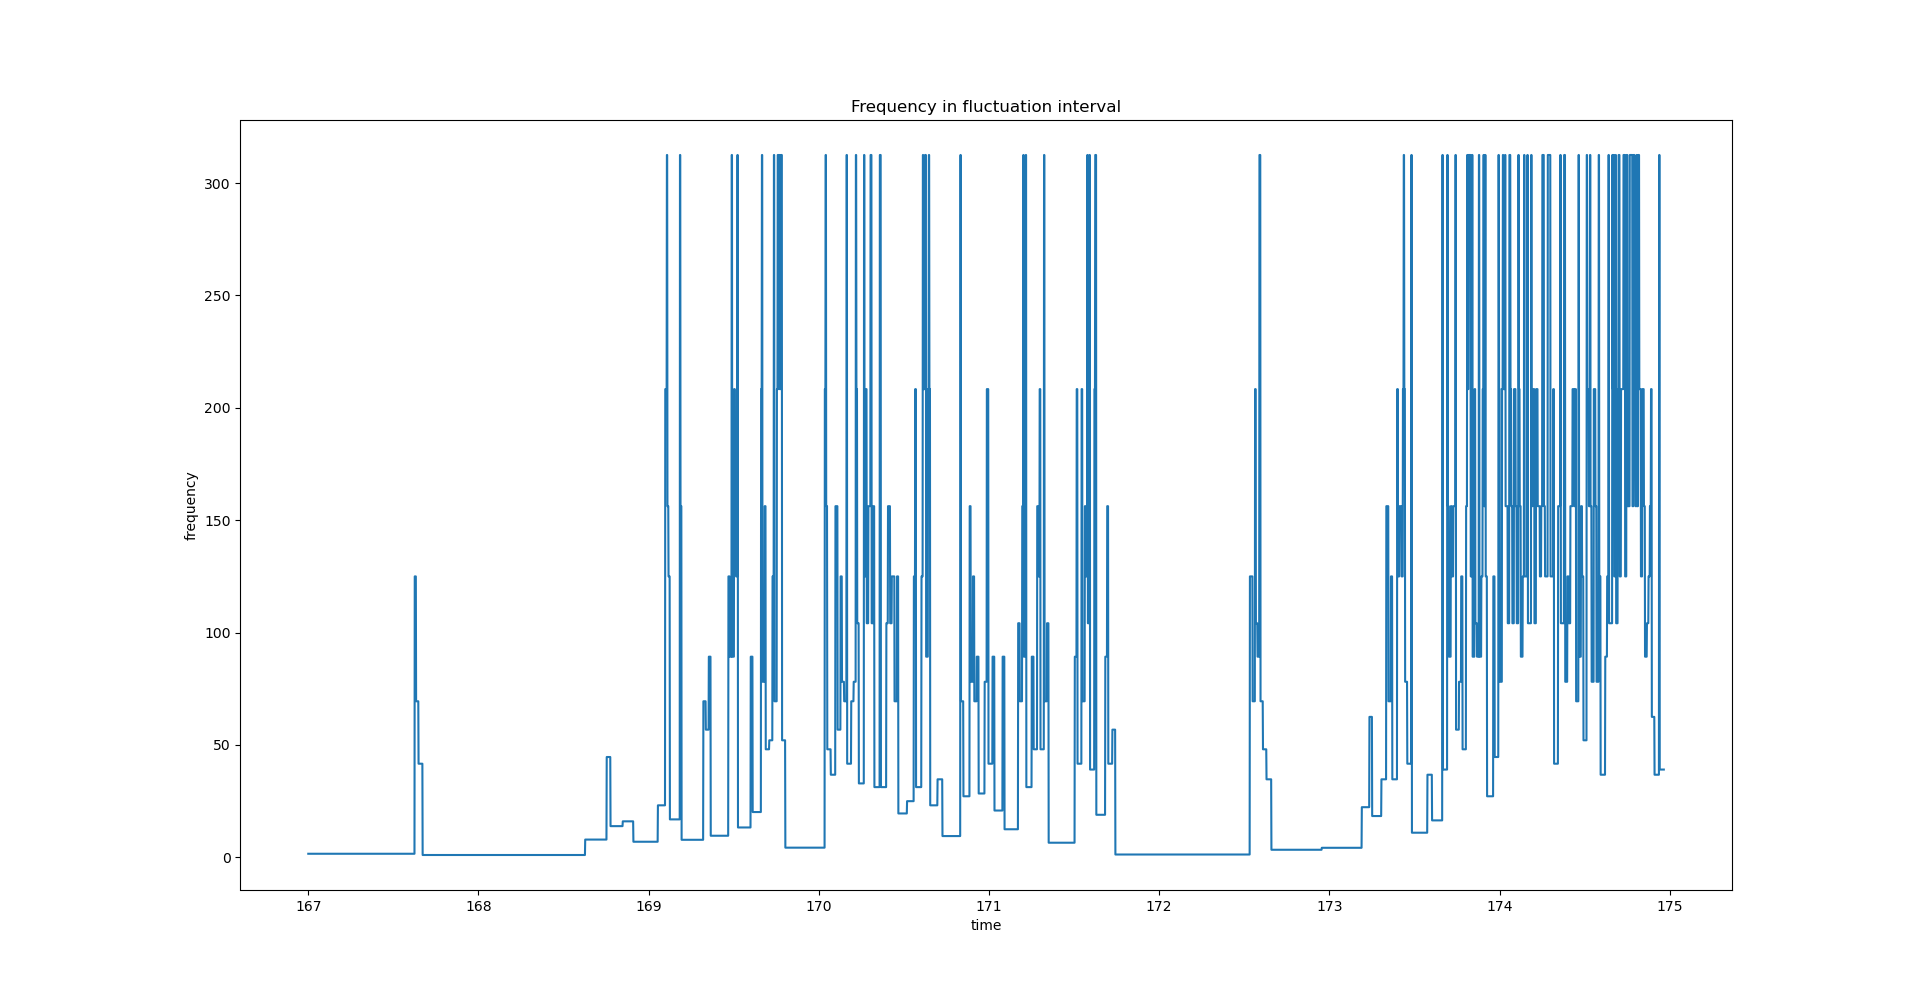
\includegraphics[width = 18cm, height = 12cm]{Fluct_dropped.png}
		\caption{Частота вращения системы на интервале колебаний [167.0, 175.0]}
		\label{fig:fluct_dropped}
	\end{figure}

	\begin{table}[H]
		\caption{Выборочные характеристики частоты вращения}
		\label{tab:my_label3}
		\begin{center}
			\vspace{5mm}
			\begin{tabular}{|c|c|c|}
				\hline
				& Среднее & Медиана\\
				\hline
				Вращение & $ 26.35 $ & $ 15.63 $\\
				\hline
				Колебания & $ 48.83 $ & $ 10.97 $\\
				\hline
			\end{tabular}
		\end{center}
	\end{table}

	Коэффициент корреляции Пирсона между частотой вращения и временем на интервале вращения $r = 0.2823$, на интервале колебаний $r = 0.4313$.
	\newline Как видим, среднее и медианное значение частоты сильно возросло, особенно в случае колебаний, что лучше отражает наблюдаемую на видео динамику. Так же виден заметный рост коэффициента корреляции.
	
	\subsection{Частота вращения системы после сильной фильтрации}
	Второй подход исходит из предположения, что само ядро в достаточной степени подвижно и хорошо выражает общую динамику движения системы, а статичность возникает в результате влияния шумовых значений. Тогда, чтобы усилить влияние ядра производится  фильтрация значений ниже 75-го перцентиля.
	\begin{figure}[H]
		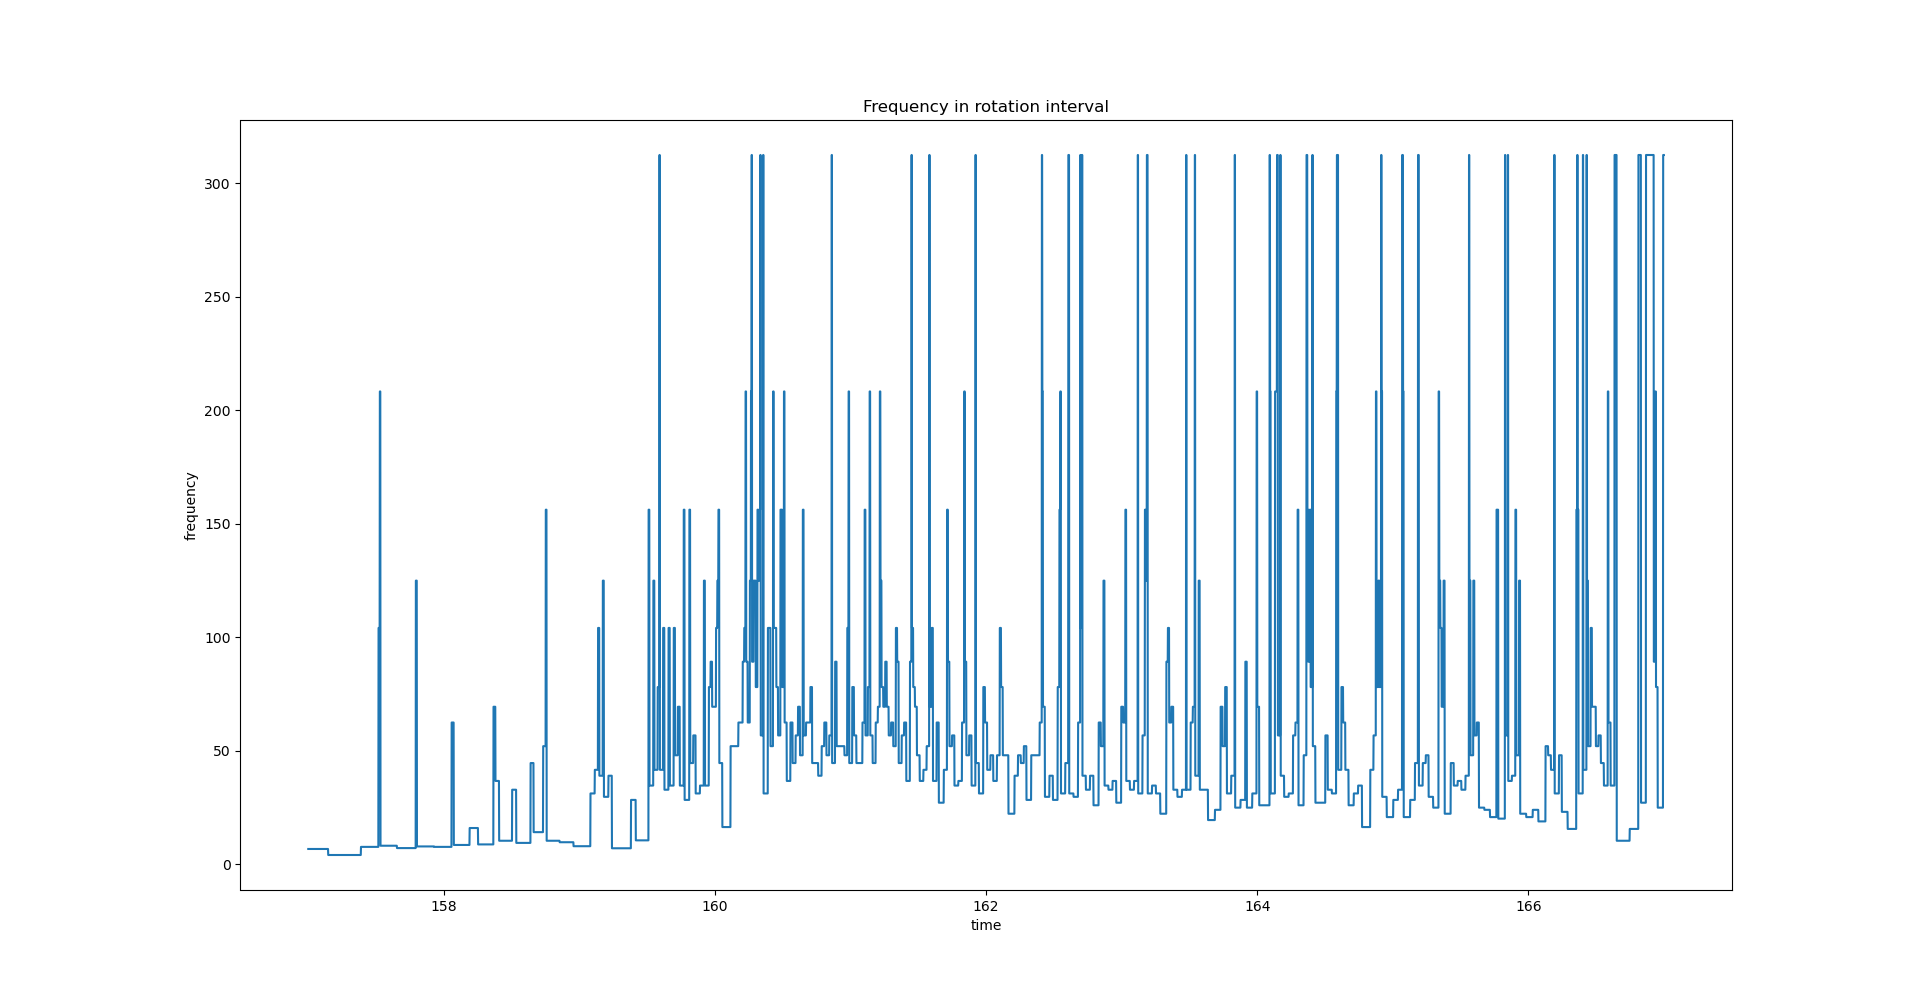
\includegraphics[width = 18cm, height = 12cm]{Rot_filtered.png}
		\caption{Частота вращения системы на интервале вращения [157.0, 167.0]}
		\label{fig:rot_filtered}
	\end{figure}
	\begin{figure}[H]
		
		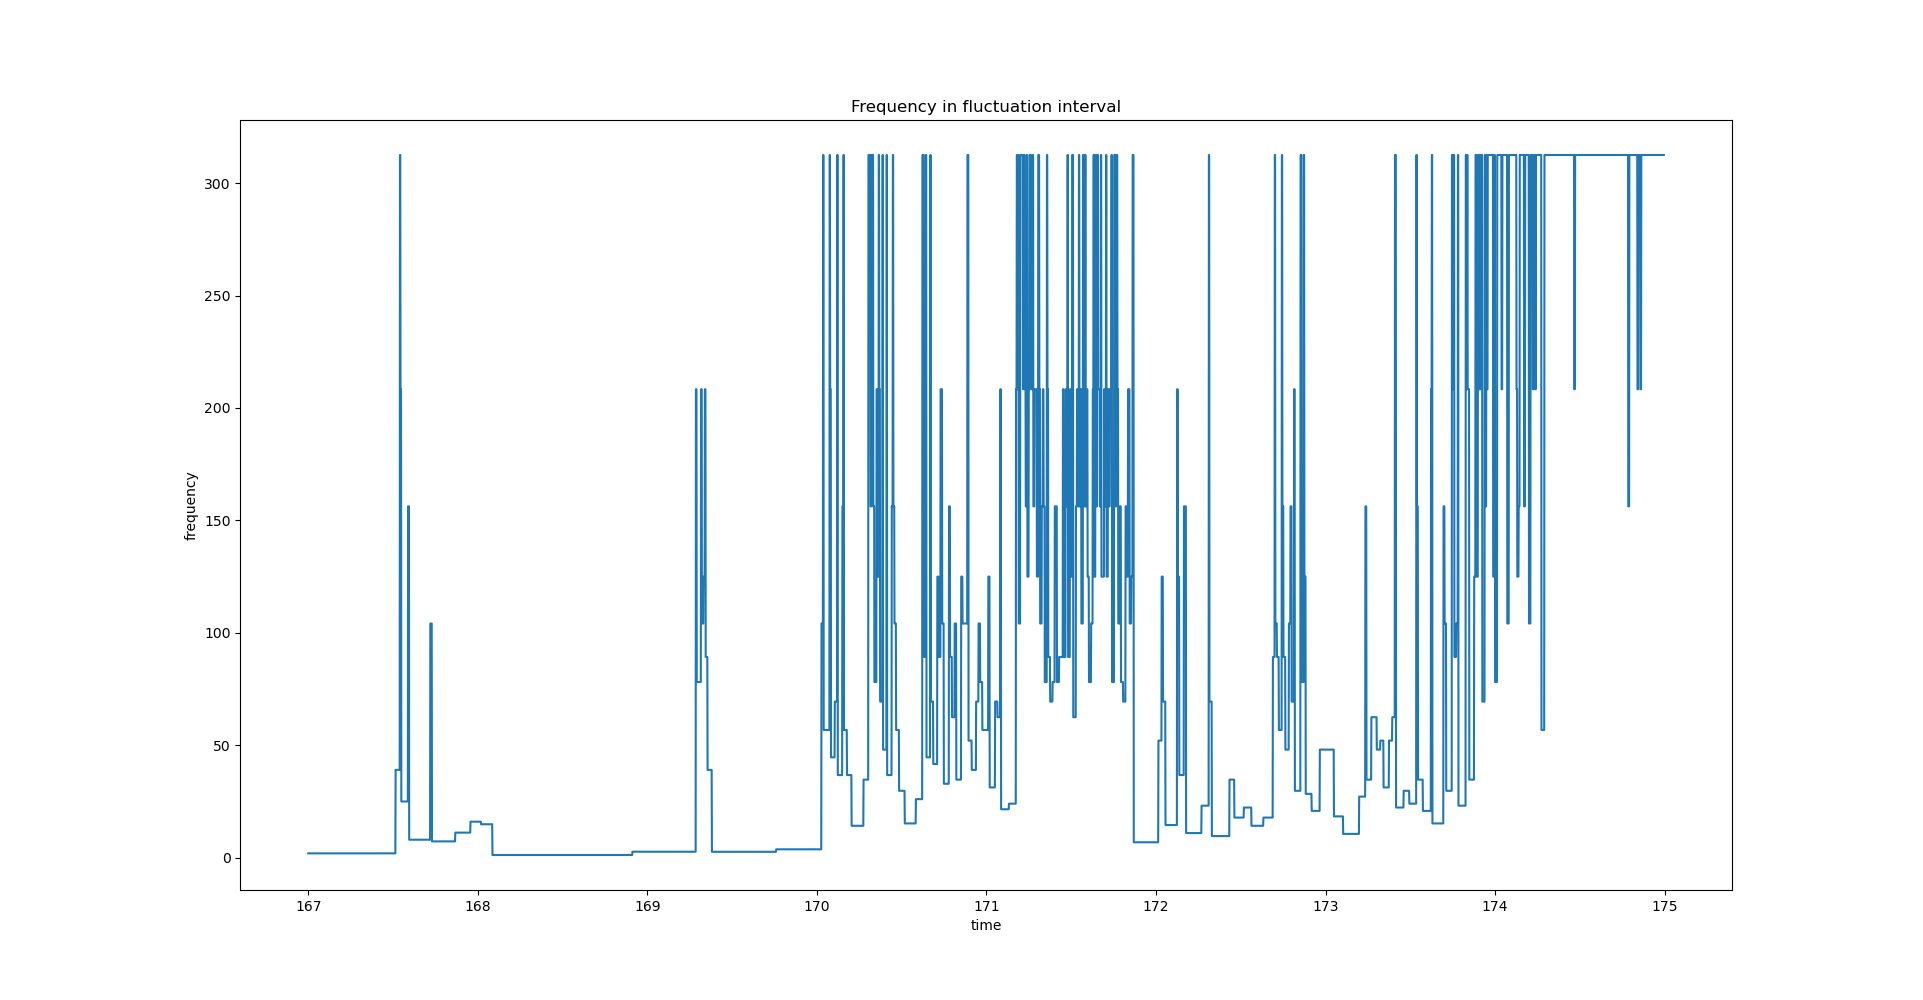
\includegraphics[width = 18cm, height = 12cm]{Fluct_filtered.png}
		\caption{Частота вращения системы на интервале колебаний [167.0, 175.0]}
		\label{fig:fluct_filtered}
	\end{figure}
	
	\begin{table}[H]
		\caption{Выборочные характеристики частоты вращения}
		\label{tab:my_label4}
		\begin{center}
			\vspace{5mm}
			\begin{tabular}{|c|c|c|}
				\hline
				& Среднее & Медиана\\
				\hline
				Вращение & $ 46.1 $ & $ 32.89 $\\
				\hline
				Колебания & $ 78.66 $ & $ 22.32 $\\
				\hline
			\end{tabular}
		\end{center}
	\end{table}
	
	Коэффициент корреляции Пирсона между частотой вращения и временем на интервале вращения $r = 0.2503$, на интервале колебаний $r = 0.6187$.
	\newline После сильной фильтрации видно, что графики стали значительно лучше отражать наблюдаемую на видео динамику. С графика интервала вращения практически исчезли частотные плато, они присутствуют только в начале, когда система ещё не перешла в фазу активного вращения. На графике колебаний плато попрежнему присутствуют, при чем основная их часть приходиться на промежуток времени после окончания интервала вращения и начала интервала колебаний, когда на видео мы наблюдаем стабилизацию системы с последующим возникновением слабых колебательных движений. 
	\newline Также заметно и улучшение выборочных характеристик: на интервале вращения относительная разность между средним и медианным значениями уменьшилась, а в абслотном значении характеристики выросли, на интервале колебаний высокая разница между медианой и средним сохраняется, но она объективно обусловлена исходной динамикой.
	\newline Коэффициент корреляции хорошо отражает наблюдаемую динамику вращения. На интервале колебаний мы наблюдаем, как со временем устаявшаяся система переходит в небольшие колебания, с наростанием частоты этих колебаний. На промежутке [162,163.5] происходит некоторое замедление, после чего колебания вновь усиливаются. На интервале вращения частота имеет явно нелинейную циклическую динамику, в результате чего коэффициент линейной корреляции Пирсона достаточно низок. 
	\section{Обсуждение}
	Исходя из полученных результатов можно сделать вывод о том, что подход, основанный на сильной фильтрации является наиболее предпочтительным при иследовании движения светимости. 
	\newline Динамика вращения системы на интервалах вращения и колебания сильно отличается: на интервале вращения [157,167] мы наблюдаем достаточно равномерные циклические колебания частоты со средним значением $46.1$ 1/мс, после чего система приходит [167,170] в устойчивое состояние, в котором центр масс практически не меняет своего положения, из которого система переходит в состояние быстрых коротких колебаний [170,175] с возростающей динамикой частоты со средним значением частоты $78.66$ 1/мс.
	\section{Приложения}
	Код программы и полученные видео на GitHub, URL:
	\url{https://github.com/dkamianskii/MatStatLabs/tree/master/Course%20Project}
	\newline Полученные видео:
	\begin{enumerate}
		\item Изменение проекции светимости по времени - projections\_in\_area
		\item Проекции светимости после удаления элементов ядра - projections\_dropped\_rot, projections\_dropped\_fluct
		\item Проекции светимости после сильной фильтрации - projections\_filtered
		\item Изменение центра масс системы по времени - centers\_mass
	\end{enumerate}
	\begin{thebibliography}{99}
		\bibitem{max}   Вероятностные разделы математики. Учебник для бакалавров технических направлений.//Под ред. Максимова Ю.Д. — Спб.: «Иван Федоров», 2001. — 592 c., илл.
		\bibitem{tokam} Баженов А.Н., Затылкин П.А. Малоракурсная реконструкция светимости плазмы для сферического токамака. Вычислительные технологии. 2020; 25(1):5–38.
	\end{thebibliography}
\end{document}